\subsection{Forward Stepwise Selection}

The first method applied is the \textit{Forward Stepwise Selection}. In particular, the algorithm variant employed uses the \textit{p-value} as entrance criterion and the AIC as comparison metric between models. The model obtained is shown in \Fig~\ref{fig:ForwardModelSummary}.
\begin{figure}[h]
	\centering
	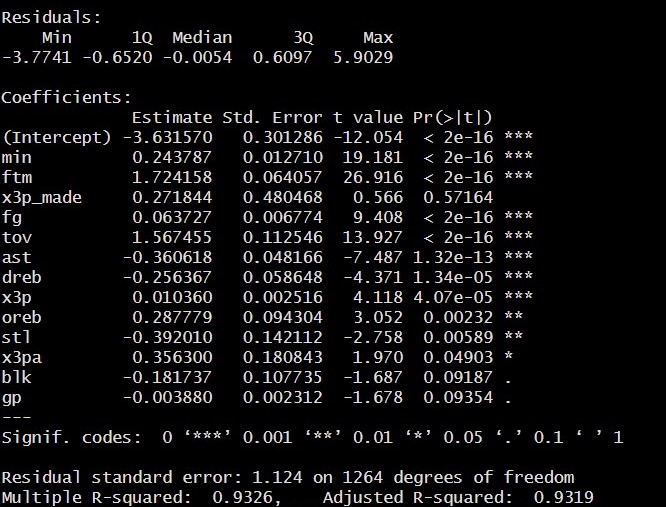
\includegraphics[width=0.35\linewidth]{ImageFiles/Regression/Forward/ForwardModelSummary}
	\caption{Forward Stepwise Selection Output Model.}
	\label{fig:ForwardModelSummary}
\end{figure}

As expected, \textit{"MIN"} and \textit{"FTM"} are included, which resulted to be important from the preliminary analysis as well. However, there are three variables that are not significantly different from 0, with \textit{p-value} threshold of $5\%$.

\vspace{0.2cm}
\noindent
\textbf{Bootstrap Statistical Inference}

On the obtained model we used the \textit{Bootstrap} technique in order to perform statistical inference on the model coefficients. In \Fig~\ref{fig:ForwardModelSummary} it is possible to see the results, that are coherent with the previous ones. This also shows that the Gaussian approximation for the error is valid in this case.
\begin{figure}[h]
	\centering
	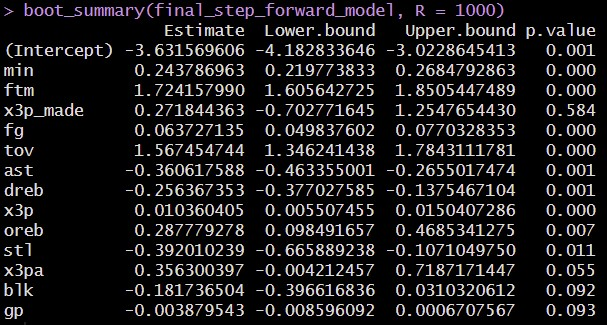
\includegraphics[width=0.4\linewidth]{ImageFiles/Regression/Forward/BootForwardModel}
	\caption{Boostrap results on Forward Stepwise Selection Output Model.}
	\label{fig:BootForwardModel}
\end{figure}

\vspace{0.2cm}
\noindent
\textbf{Final Forward Model}

The final Forward Model, shown in \Fig~\ref{fig:ForwardFinalModelSummary}, is obtained removing the non significant variables. Instead, in \Fig~\ref{fig:ForwardFinalModelResiduals} and \Fig~\ref{fig:ForwardFinalModelResidualsDist} it is possible to see plots of the residuals, that have a Gaussian shape with 0 mean. This means that the model is likely adequate for our purposes.

\begin{figure}[h]
	\centering
	\begin{subfigure}{.6\textwidth}
		\centering
		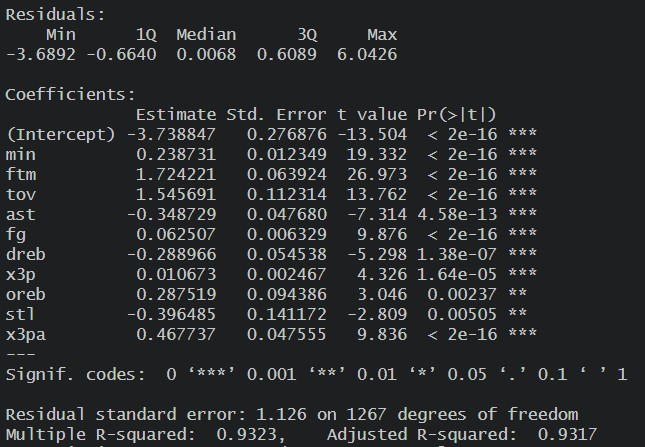
\includegraphics[width=0.5\linewidth]{ImageFiles/Regression/Forward/ForwardFinalModelSummary}
		\caption{Forward Stepwise Selection Model Summary.}
		\label{fig:ForwardFinalModelSummary}
	\end{subfigure}
	\begin{subfigure}{.6\textwidth}
		\centering
		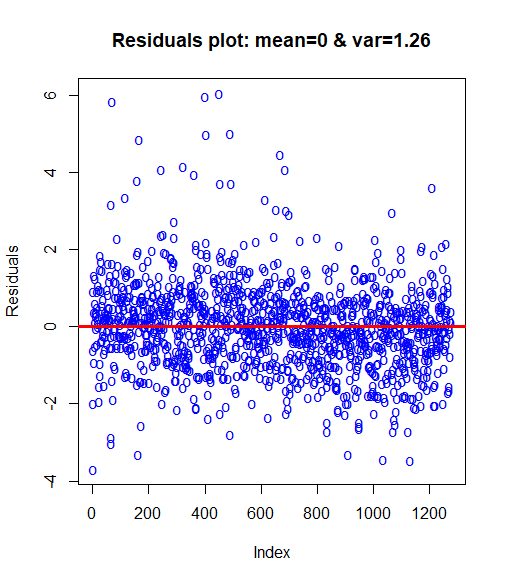
\includegraphics[width=0.5\linewidth]{ImageFiles/Regression/Forward/ForwardFinalModelResiduals}
		\caption{Forward Stepwise Selection Model Residuals.}
		\label{fig:ForwardFinalModelResiduals}
	\end{subfigure}%
	\begin{subfigure}{.6\textwidth}
		\centering
		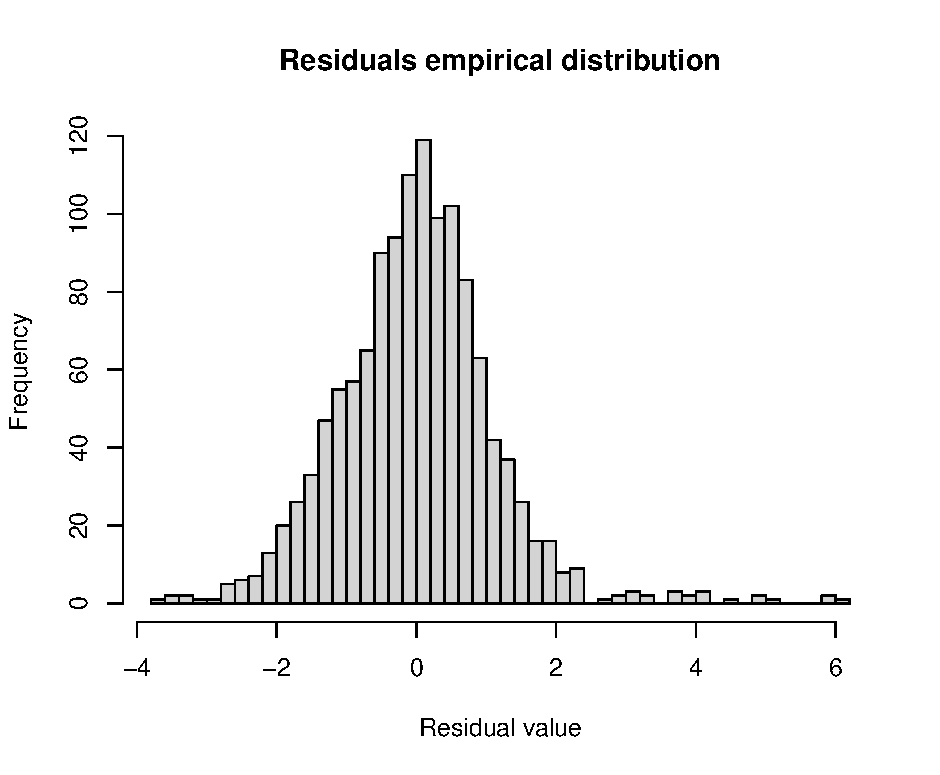
\includegraphics[width=0.5\linewidth]{ImageFiles/Regression/Forward/ForwardFinalModelResidualsDist}
		\caption{Forward Stepwise Selection Model Residuals.}
		\label{fig:ForwardFinalModelResidualsDist}
	\end{subfigure}
	\caption{The final Forward Stepwise Selection Model.}
	\label{fig:FinalFSSM}
\end{figure}

